\section*{Conclusione}
I risultati esposti in precedenza hanno evidenziato come sia per l'albume che per il tuorlo siano presenti impurità.
Nel primo caso è plausibile che tale impurità sia presente solo in piccole dosi, vista la scarsa intensità del segnale; mentre nel secondo caso è supponibile che il tuorlo sia costituito da più composti.

Per dare un'ulteriore solidità a tale risultato si consideri il grafico \ref{fig:SigT_Sig}. 
Da questo tipo di illustrazione è possibile valutare quanto i campioni siano descritti da un andamento monoesponenziale e quindi siano costituiti da un solo componente.

Le curve relative ai tempi di rilassamento dell'albume descrivono un andamento lineare finchè il segnale non ha intensità pari a quella del rumore. 
Ciò implica che l'effetto più rilevante è dato dal singolo costituente dell'albume e l'effetto dato dall'impurità è trascurabile, confermando la leggera presenza ipotizzata precedentemente.

Riguardo al tuorlo invece è possibile notare che per entrambi i tempi di rilassamento si ha un andamento che approssima inizialmente una retta ma che rapidamente si inclina per formare una curva.
Ciò rafforza l'idea che il tuorlo non sia costituito da un solo composto ma da diversi.

\begin{figure}[h]
\centering
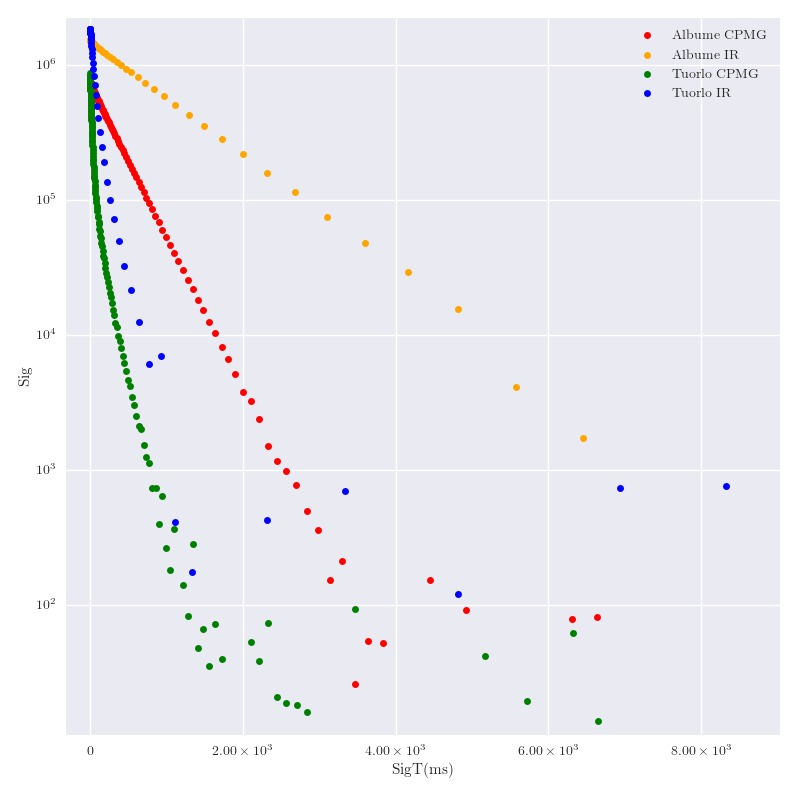
\includegraphics[scale=0.3]{SigT_Sig.jpeg}
\caption{Rappresentazione semilogaritmica della relazione tra l'intensità del segnale acquisito e il tempo di acquisizione.}
\label{fig:SigT_Sig}
\end{figure}


Oltre a valutare la composizione di albume e tuorlo, è possibile dedurre dai risultati della sezione precedente che il contrasto che si può ottenere tra immagini pesato in $T_1$ e $T_2$ è alto per entrambi i campioni.
Infatti, per ognuno dei due si hanno tempi di rilassamento $T_2$ molto inferiori a $T_1$.

Avendo ottenuto i valori di $T_1$ e $T_2$ per il tuorlo e per l'albume, è ora possibile sfruttare la formula seguente di MRI Spin-Echo con metodo spin warp per calcolare gli intervalli di $T_E$ e $T_R$ per ricavare immagini pesate.

${M_y}_{(T_R,T_E)} = M_0[1-e^{-\frac{T_R}{T_1}}(2e^{-\frac{T_{E/2}}{T_1}}-1)]e^{-\frac{T_E}{T_2}}$		\\
	

La tabella seguente contiene gli intervalli derivati.


\begin{table}[h]
	\centering
	\begin{tabular}{ccc}
	\toprule
		\textbf{Pesate in $T_1$} &	\textbf{Pesate in $T_2$}	\\
	\midrule
		$T_E = 50\,ms$			&		$T_E = 16\,ms$	 \\	
		$T_R = 1000\,ms$			&		$T_R = 400\,ms$ \\
	\bottomrule
	\end{tabular}
	\caption{Stime degli intervalli per $T_E$ e $T_R$ per generare immagini MRI pesate.}	
	\label{tab:Pesate}
\end{table}